\documentclass[12pt, a4paper]{article}

% ─── PACKAGES ────────────────────────────────────────────────────────────────
\usepackage[T1]{fontenc}
\usepackage[utf8]{inputenc}
\usepackage{lmodern}
\usepackage[english]{babel}
\usepackage{geometry}
\usepackage{graphicx}
\usepackage{microtype}
\usepackage{setspace}
\usepackage{titlesec}
\usepackage{fancyhdr}
\usepackage{hyperref}
\usepackage{xcolor}
\usepackage{amsmath, amssymb}
\usepackage{listings}
\usepackage{booktabs}
\usepackage{caption}
\usepackage{subcaption}
\usepackage{float}
\usepackage{csquotes}
\usepackage{tocloft}
\usepackage{parskip}
\usepackage{tabularx}
\usepackage[style=ieee, backend=biber]{biblatex}
\usepackage{tcolorbox}
\newtcolorbox{infobox_env}{
  colback=gray!5,
  colframe=gray!75!black,
  boxrule=0.5pt,
  arc=4pt
}

% ─── PAGE GEOMETRY ───────────────────────────────────────────────────────────
\geometry{
  a4paper,
  top=2.5cm,
  bottom=2.5cm,
  left=3cm,
  right=2.5cm,
  headheight=14pt
}

% ─── COLORS ──────────────────────────────────────────────────────────────────
\definecolor{unipd-red}{RGB}{155, 0, 20}   % UNIPD institutional red
\definecolor{code-bg}{RGB}{245, 245, 245}
\definecolor{code-gray}{RGB}{100, 100, 100}

% ─── HYPERREF SETUP ──────────────────────────────────────────────────────────
\hypersetup{
  colorlinks = true,
  linkcolor  = unipd-red,
  citecolor  = unipd-red,
  urlcolor   = unipd-red,
  pdftitle   = {NVIDIAScape: Container Escape via LD\_PRELOAD Injection},
  pdfauthor  = {Alessio Demo},
}

% ─── SECTION FORMATTING ──────────────────────────────────────────────────────
\titleformat{\section}
  {\large\bfseries\color{unipd-red}}
  {\thesection}{1em}{}[\titlerule]

\titleformat{\subsection}
  {\normalsize\bfseries}
  {\thesubsection}{1em}{}

\titleformat{\subsubsection}
  {\normalsize\itshape}
  {\thesubsubsection}{1em}{}

% ─── HEADER / FOOTER ─────────────────────────────────────────────────────────
\pagestyle{fancy}
\fancyhf{}
\fancyhead[L]{\small\textit{NVIDIAScape: Container Escape via LD\_PRELOAD Injection}}
\fancyhead[R]{\small\textit{Alessio Demo}}
\fancyfoot[C]{\thepage}
\renewcommand{\headrulewidth}{0.4pt}

% ─── CODE LISTING STYLE ──────────────────────────────────────────────────────
\lstdefinestyle{mycode}{
  backgroundcolor = \color{code-bg},
  basicstyle      = \ttfamily\footnotesize,
  breaklines      = true,
  captionpos      = b,
  commentstyle    = \color{code-gray}\itshape,
  keywordstyle    = \color{unipd-red}\bfseries,
  stringstyle     = \color{teal},
  numberstyle     = \tiny\color{code-gray},
  numbers         = left,
  numbersep       = 8pt,
  frame           = single,
  framerule       = 0.4pt,
  rulecolor       = \color{code-gray},
  tabsize         = 4,
  showstringspaces= false,
}
\lstset{style=mycode}

% ─── LINE SPACING ────────────────────────────────────────────────────────────
\onehalfspacing

% ─── TOC STYLING ─────────────────────────────────────────────────────────────
\renewcommand{\cftsecfont}{\bfseries}
\renewcommand{\cftsecpagefont}{\bfseries}
\setlength{\cftbeforesecskip}{4pt}


% ─── Bibliography ─────────────────────────────────────────────────────────────
\addbibresource{ref.bib}
% ═════════════════════════════════════════════════════════════════════════════
%  DOCUMENT START
% ═════════════════════════════════════════════════════════════════════════════
\begin{document}

% ─── TITLE PAGE ──────────────────────────────────────────────────────────────
% ─── TITLE PAGE ──────────────────────────────────────────────────────────────
\begin{titlepage}
  \thispagestyle{empty}

  % ── Top block: logo + university info ──────────────────────────────────────
  \begin{minipage}[t]{0.20\textwidth}
    \vspace{0pt}
    
\includegraphics[width=\linewidth]{images/unipd-logo.png}
  \end{minipage}
  \hfill
  \begin{minipage}[t]{0.78\textwidth}
    \vspace{4pt}
    {\large University of Padua}\\
    {\large\textbf{Department of Information Engineering}}\\[4pt]
    \rule{\linewidth}{0.5pt}\\[6pt]
    {\large Master Degree in Computer Engineering}
  \end{minipage}

  \vspace{0pt plus 0.8fill}   % <-- sostituisce il primo \vfill

  % ── Essay label + title block ─────────────────────────────────────────────
  \begin{flushleft}
    {\large Computer \& Networks Security essay}\\[0.4cm]
    {\LARGE\bfseries\color{unipd-red}
      NVIDIAScape: Container Escape via LD\_PRELOAD Injection
    \par}
    \vspace{0.4cm}
    {\large May 2026}
  \end{flushleft}

  \vspace{0pt plus 1.2fill}

  % ── Candidate / Supervisor block ───────────────────────────────────────────
  \noindent
  \begin{minipage}[b]{0.45\textwidth}
    {\large Candidate:}\\[2pt]
    {\large Alessio Demo}\\
    {\large Student ID: 2142885}
  \end{minipage}
  \hfill
  \begin{minipage}[b]{0.45\textwidth}
    \raggedleft
    {\large Professor:}\\[2pt]
    {\large Mauro Migliardi}
  \end{minipage}

\end{titlepage}

% ─── ABSTRACT ────────────────────────────────────────────────────────────────
\newpage
\thispagestyle{plain}
\begin{center}
  {\large\bfseries Abstract}
\end{center}
\noindent
This essay analyses \textbf{NVIDIAScape} (CVE-2025-23266), a container-escape
vulnerability affecting the NVIDIA Container Toolkit. The attack exploits the
\texttt{LD\_PRELOAD} environment variable, injected from inside a container,
to force a privileged host-side hook to load attacker-controlled
shared libraries. The root cause lies in the unsafe inheritance of the container
environment by a process running with root privileges on the host, in violation of
the principle of least privilege and proper isolation boundaries. The paper also describes the attack surface, the exploitation chain, the underlying design flaws, and the remediation measures introduced by NVIDIA and the broader container-security ecosystem.

% ─── TABLE OF CONTENTS ───────────────────────────────────────────────────────
\newpage
\tableofcontents

% ─── MAIN BODY ───────────────────────────────────────────────────────────────
\newpage
\section{Introduction}
\label{sec:intro}

The rapid proliferation of containerized workloads has transformed the way computational resources are packaged, deployed, and shared across modern infrastructure.
In particular we are talking about Containers, but what are they?\\
\textbf{Containers} are lightweight and portable execution environments built upon Linux kernel primitives such as namespaces, control groups, and security computer facilities, and in the last years have become the main deployment unit for cloud-native applications, data processing pipelines, artificial intelligence and machine learning workloads \cite{sultan2019container}.
The emergence of large-scale AI training and inference has introduced a new and critical dimension to this landscape: the need to share hardware accelerators, most prominently \textbf{NVIDIA Graphics Processing Units (GPUs)}, across multiple isolated container workloads.
Unlike CPU resources, which are abstracted transparently by the kernel scheduler, GPU access requires deep integration between the container runtime and the host operating system's driver stack \cite{nvidia_ctk_docs}. This integration is precisely where the attack surface examined in this paper resides.
Going into details: The \textbf{NVIDIA Container Toolkit} (\texttt{nvidia-ctk}) is the software layer responsible for exposing GPU capabilities to containerised processes \cite{nvidia_ctk_github}.
It acts as a privileged extension of the container runtime, executing hooks with root privileges on the host to configure the necessary device mappings and library bindings before the container process starts; the negative side of things is that it can be fatally exploited when the privileged process fails to sanitise the environment it inherits from an untrusted source.
This vulnerability is identified as \textbf{CVE-2025-23266} \cite{nvd_cve_2025_23266} and allows a process running inside a container (potentially an unprivileged tenant in a shared cloud environment) to inject the \texttt{LD\_PRELOAD} environment variable into the execution context of the host-side hook.
Because the Linux dynamic linker processes \texttt{LD\_PRELOAD} variable before any application code runs \cite{linux_ldso_manpage}, the attacker's malicious shared library is loaded and executed with full root privileges on the host, achieving a complete container escape.
The significance of this vulnerability extends beyond its technical elegance. It strikes at a foundational assumption of container security: that isolation primitives reliably prevent a containerised process from affecting the host \cite{lin2018measurement}. In the context of multi-tenant AI cloud services ( where numerous organisations share the same physical GPU nodes ) a single exploitable container can compromise the entire host, potentially exposing sensitive model weights, training data, and API keys.

\newpage
\medskip
\noindent This paper is structured as follows:
\begin{itemize}
    \item Chapter \ref{sec:background} provides the necessary background on Linux container security, the NVIDIA Container Toolkit, the \texttt{LD\_PRELOAD} mechanism, and historically related vulnerabilities.
    \item Chapter \ref{sec:vuln} presents a deep technical analysis of CVE-2025-23266 itself.
    \item Chapter \ref{sec:exploitation} details the exploitation mechanics step by step.
    \item Chapter \ref{sec:impact} assesses the real-world impact.
    \item Chapter \ref{sec:mitigation} discusses mitigations and hardening strategies.
    \item Chapter \ref{sec:implications} reflects on broader security implications.
\end{itemize}    

\newpage
\section{Background and Related Work}
\label{sec:background}

% ~4.000 characters total across subsections

\subsection{Linux Containers and Isolation Primitives}
\label{subsec:containers}

Modern Linux containers do not rely on a distinct kernel or hardware boundary as virtual machines do. Instead, they exploit a layered set of kernel features to create the \textit{illusion} of isolation while sharing the same underlying kernel with the host \cite{sultan2019container}.

\paragraph{Namespaces.} Linux namespaces partition global resources into per-process views \cite{linux_namespaces_manpage}. The key namespaces for container isolation are: \texttt{pid} (process identifiers), \texttt{net} (network stack), \texttt{mnt} (filesystem mount points), \texttt{uts} (hostname and domain name), \texttt{ipc} (inter-process communication), and \texttt{user} (user and group identifiers). A process confined within these namespaces cannot observe or interact with resources belonging to other namespaces.

\paragraph{Control Groups (cgroups).} Cgroups enforce resource accounting and limits — CPU time, memory, I/O bandwidth, and device access. They do not provide security isolation, but prevent resource exhaustion attacks and can restrict device access via the \texttt{devices} cgroup controller.

\paragraph{Seccomp.} The Secure Computing Mode (\texttt{seccomp}) allows fine-grained filtering of system calls. Container runtimes like Docker apply a default seccomp profile that blocks hundreds of potentially dangerous syscalls from within the container.

\paragraph{Capabilities.} Linux capabilities decompose the monolithic root privilege into discrete units (e.g., \texttt{CAP\_NET\_ADMIN}, \texttt{CAP\_SYS\_PTRACE}) \cite{linux_capabilities_manpage}. Containers typically run with a reduced capability set, preventing common privilege escalation techniques that require specific capabilities.
These primitives form a defence-in-depth stack \cite{lin2018measurement, nist_sp800_190}, however their security guarantees are only as strong as the correctness of the kernel implementation and the integrity of the privileged processes that configure and manage the container lifecycle.
When a privileged process outside the container namespace interacts with untrusted input from within it (as in the case of NVIDIAScape) the isolation boundary can be subverted without any kernel vulnerability being required.

\subsection{The NVIDIA Container Toolkit}
\label{subsec:nvidia-ctk}

The NVIDIA Container Toolkit is an open-source project that enables NVIDIA GPU access for containerised workloads \cite{nvidia_ctk_github}. It consists of several components:
\begin{itemize}
  \item \textbf{libnvidia-container}: A shared library that performs the actual GPU device configuration.
  \item \textbf{nvidia-container-runtime}: A wrapper around standard OCI-compatible runtimes (e.g., \texttt{runc}) that injects NVIDIA-specific configuration.
  \item \textbf{nvidia-ctk}: The CLI tool and hook binary used to configure GPU access at container startup.
\end{itemize}
The toolkit integrates with the Open Container Initiative (OCI) specification through the \textbf{OCI hook} mechanism \cite{oci_runtime_spec, oci_image_spec}. OCI hooks are executable programs invoked by the container runtime at defined lifecycle points — \texttt{prestart}, \texttt{createRuntime}, \texttt{poststart}, and \texttt{poststop}. The NVIDIA \texttt{prestart} hook runs \textit{on the host}, with root privileges, before the container process starts. Its role is to mount the necessary NVIDIA device files and libraries into the container's filesystem \cite{nvidia_ctk_docs}.

Critically, the hook process is spawned in a context that inherits environmental information from the container's configuration. As we shall examine in detail, this inheritance is the root cause of CVE-2025-23266.
 
\begin{infobox_env}
The OCI hook specification (\textit{runtime-spec}) does not mandate environment sanitisation for hook executables \cite{oci_runtime_spec}. The security burden is implicitly placed on hook implementors, who must explicitly clean their execution environment when operating with elevated privileges.
\end{infobox_env}

\subsection{The Dynamic Linker and \texttt{LD\_PRELOAD}}
\label{subsec:ldpreload}

The Linux dynamic linker (\texttt{ld.so} / \texttt{ld-linux.so}) is responsible for loading shared libraries required by an executable at runtime \cite{linux_ldso_manpage}. It resolves symbol dependencies, maps library segments into the process address space, and transfers control to the program's entry point.
\paragraph{\texttt{LD\_PRELOAD}.} The \texttt{LD\_PRELOAD} environment variable is a feature of the dynamic linker that allows specifying one or more shared libraries to be loaded \textit{before all the others}  \cite{linux_ldso_manpage}. Its legitimate uses include debugging, profiling (e.g., replacing \texttt{malloc} with a tracking allocator), and binary instrumentation.
The security implications of \texttt{LD\_PRELOAD} are well-understood. The dynamic linker explicitly disables \texttt{LD\_PRELOAD} (and related variables such as \texttt{LD\_LIBRARY\_PATH} and \texttt{LD\_AUDIT}) when it detects that the effective user ID differs from the real user ID (the condition that characterises Set-UID programs \cite{linux_ldso_manpage}). This protection exists precisely because allowing untrusted \texttt{LD\_PRELOAD} injection into a privileged process would enable trivial privilege escalation.
However, this protection is only automatic for Set-UID binaries, in the other hand  for a process that \textit{acquires} elevated privileges through other means (such as being spawned directly by a privileged parent) and does not explicitly sanitise its environment, \texttt{LD\_PRELOAD} remains fully operative \cite{linux_execve_manpage}. This is the precise gap that NVIDIAScape exploits.

\begin{lstlisting}[language=bash, caption={The dynamic linker's LD\_PRELOAD security bypass for SUID binaries — not applicable when privilege is inherited from parent process.}]
# For a SUID binary, the linker ignores LD_PRELOAD:
$ ls -la /usr/bin/sudo
-rwsr-xr-x 1 root root ... /usr/bin/sudo
$ LD_PRELOAD=/tmp/evil.so sudo whoami
# LD_PRELOAD is silently ignored  (protection works)
 
# But for a root-spawned non-SUID hook process:
# The linker DOES honour LD_PRELOAD  (no automatic protection)
\end{lstlisting}

\subsection{Related Vulnerabilities}
\label{subsec:related-vulns}

NVIDIAScape is not an isolated incident, it belongs to a broader family of container escape vulnerabilities that share a common pattern: a privileged host-side component incorrectly trusts or inherits input from within the container boundary \cite{lin2018measurement}.

\paragraph{CVE-2024-0132 — NVIDIA Container Toolkit (2024).} A related vulnerability in an earlier version of the NVIDIA Container Toolkit allowed a crafted container image to mount sensitive host paths via time-of-check/time-of-use (TOCTOU) race conditions in the toolkit's filesystem traversal logic \cite{nvd_cve_2024_0132}\cite{wiz_nvidia_2024}. Unlike CVE-2025-23266, CVE-2024-0132 exploited filesystem handling rather than environment inheritance, but the underlying theme (insufficient trust boundary enforcement in a privileged GPU management layer) is identical.

\paragraph{Leaky Vessels (CVE-2024-21626 and related — runc, 2024).} The ``Leaky Vessels'' cluster of vulnerabilities, disclosed in January 2024, affected the \texttt{runc} container runtime \cite{nvd_cve_2024_21626} \cite{leaky_vessels_disclosure}. CVE-2024-21626 allowed an attacker to leak a file descriptor referencing the host filesystem root by exploiting the order of operations in \texttt{runc}'s process initialisation, this enabled container escape with minimal preconditions. Much like NVIDIAScape, the vulnerability required no kernel exploit (only exploitation of a privileged userspace component's incorrect handling of state that crossed the container boundary).

\paragraph{CVE-2019-5736 — runc.} An earlier critical vulnerability in \texttt{runc} allowed a malicious container to overwrite the host \texttt{runc} binary by exploiting \texttt{/proc/self/exe} references during container execution \cite{nvd_cve_2019_5736}. The attacker could then execute arbitrary code as root the next time any container was started. This vulnerability established the now well-known principle that \textit{container runtime processes themselves are attack surface}.

\paragraph{CVE-2022-0492 — cgroup v1.} This kernel vulnerability allowed container escape via \texttt{cgroup} release agent abuse when the container had a weakened security profile \cite{nvd_cve_2022_0492}. While a kernel-level vulnerability rather than a userspace toolkit flaw, it reinforces the point that GPU and system management toolkits that run without full security profiles (no AppArmor, no seccomp) remove critical layers of defence.

These precedents collectively demonstrate that privileged host-side components managing container lifecycle (whether container runtimes, GPU toolkits, or storage drivers) represent a persistent and high-value attack surface that demands rigorous security engineering \cite{sultan2019container} \cite{lin2018measurement}.

\newpage
\section{CVE-2025-23266 --- Technical Analysis}
\label{sec:vuln}

% ~6.000 characters total across subsections

\subsection{Vulnerability Description}
\label{subsec:vuln-desc}

CVE-2025-23266 is a \textbf{container escape vulnerability} in the NVIDIA Container Toolkit \cite{nvd_cve_2025_23266, nvidia_advisory_2025}. It was publicly disclosed in 2025 and assigned a CVSS v3.1 base score of \textbf{9.0 (Critical)} \cite{cvss_v31_spec}, reflecting the combination of high confidentiality, integrity, and availability impact at the host level, with the attack vector being local (within the container) but resulting in complete host compromise.

The vulnerability affects versions of the NVIDIA Container Toolkit prior to the patched release and stems from a failure to sanitise the execution environment of the \texttt{nvidia-ctk} OCI hook process. Specifically, environment variables set within the container — including \texttt{LD\_PRELOAD} — are inherited by the hook process when it is invoked by the container runtime on the host. Since the hook process runs with root privileges on the host, this inheritance allows an attacker inside the container to force the loading of an arbitrary shared library into the host's privileged process space.

\begin{infobox_env}
CVE-2025-23266 does not require any kernel vulnerability, any special container privileges (e.g., \texttt{--privileged}), or any network access. The only prerequisite is that the attacker can run a container on a host equipped with the NVIDIA Container Toolkit (a standard precondition in any GPU cloud environment).
\end{infobox_env}

Graphically we can represent the attack flow as follows:


\begin{figure}[htbp]
  \centering
  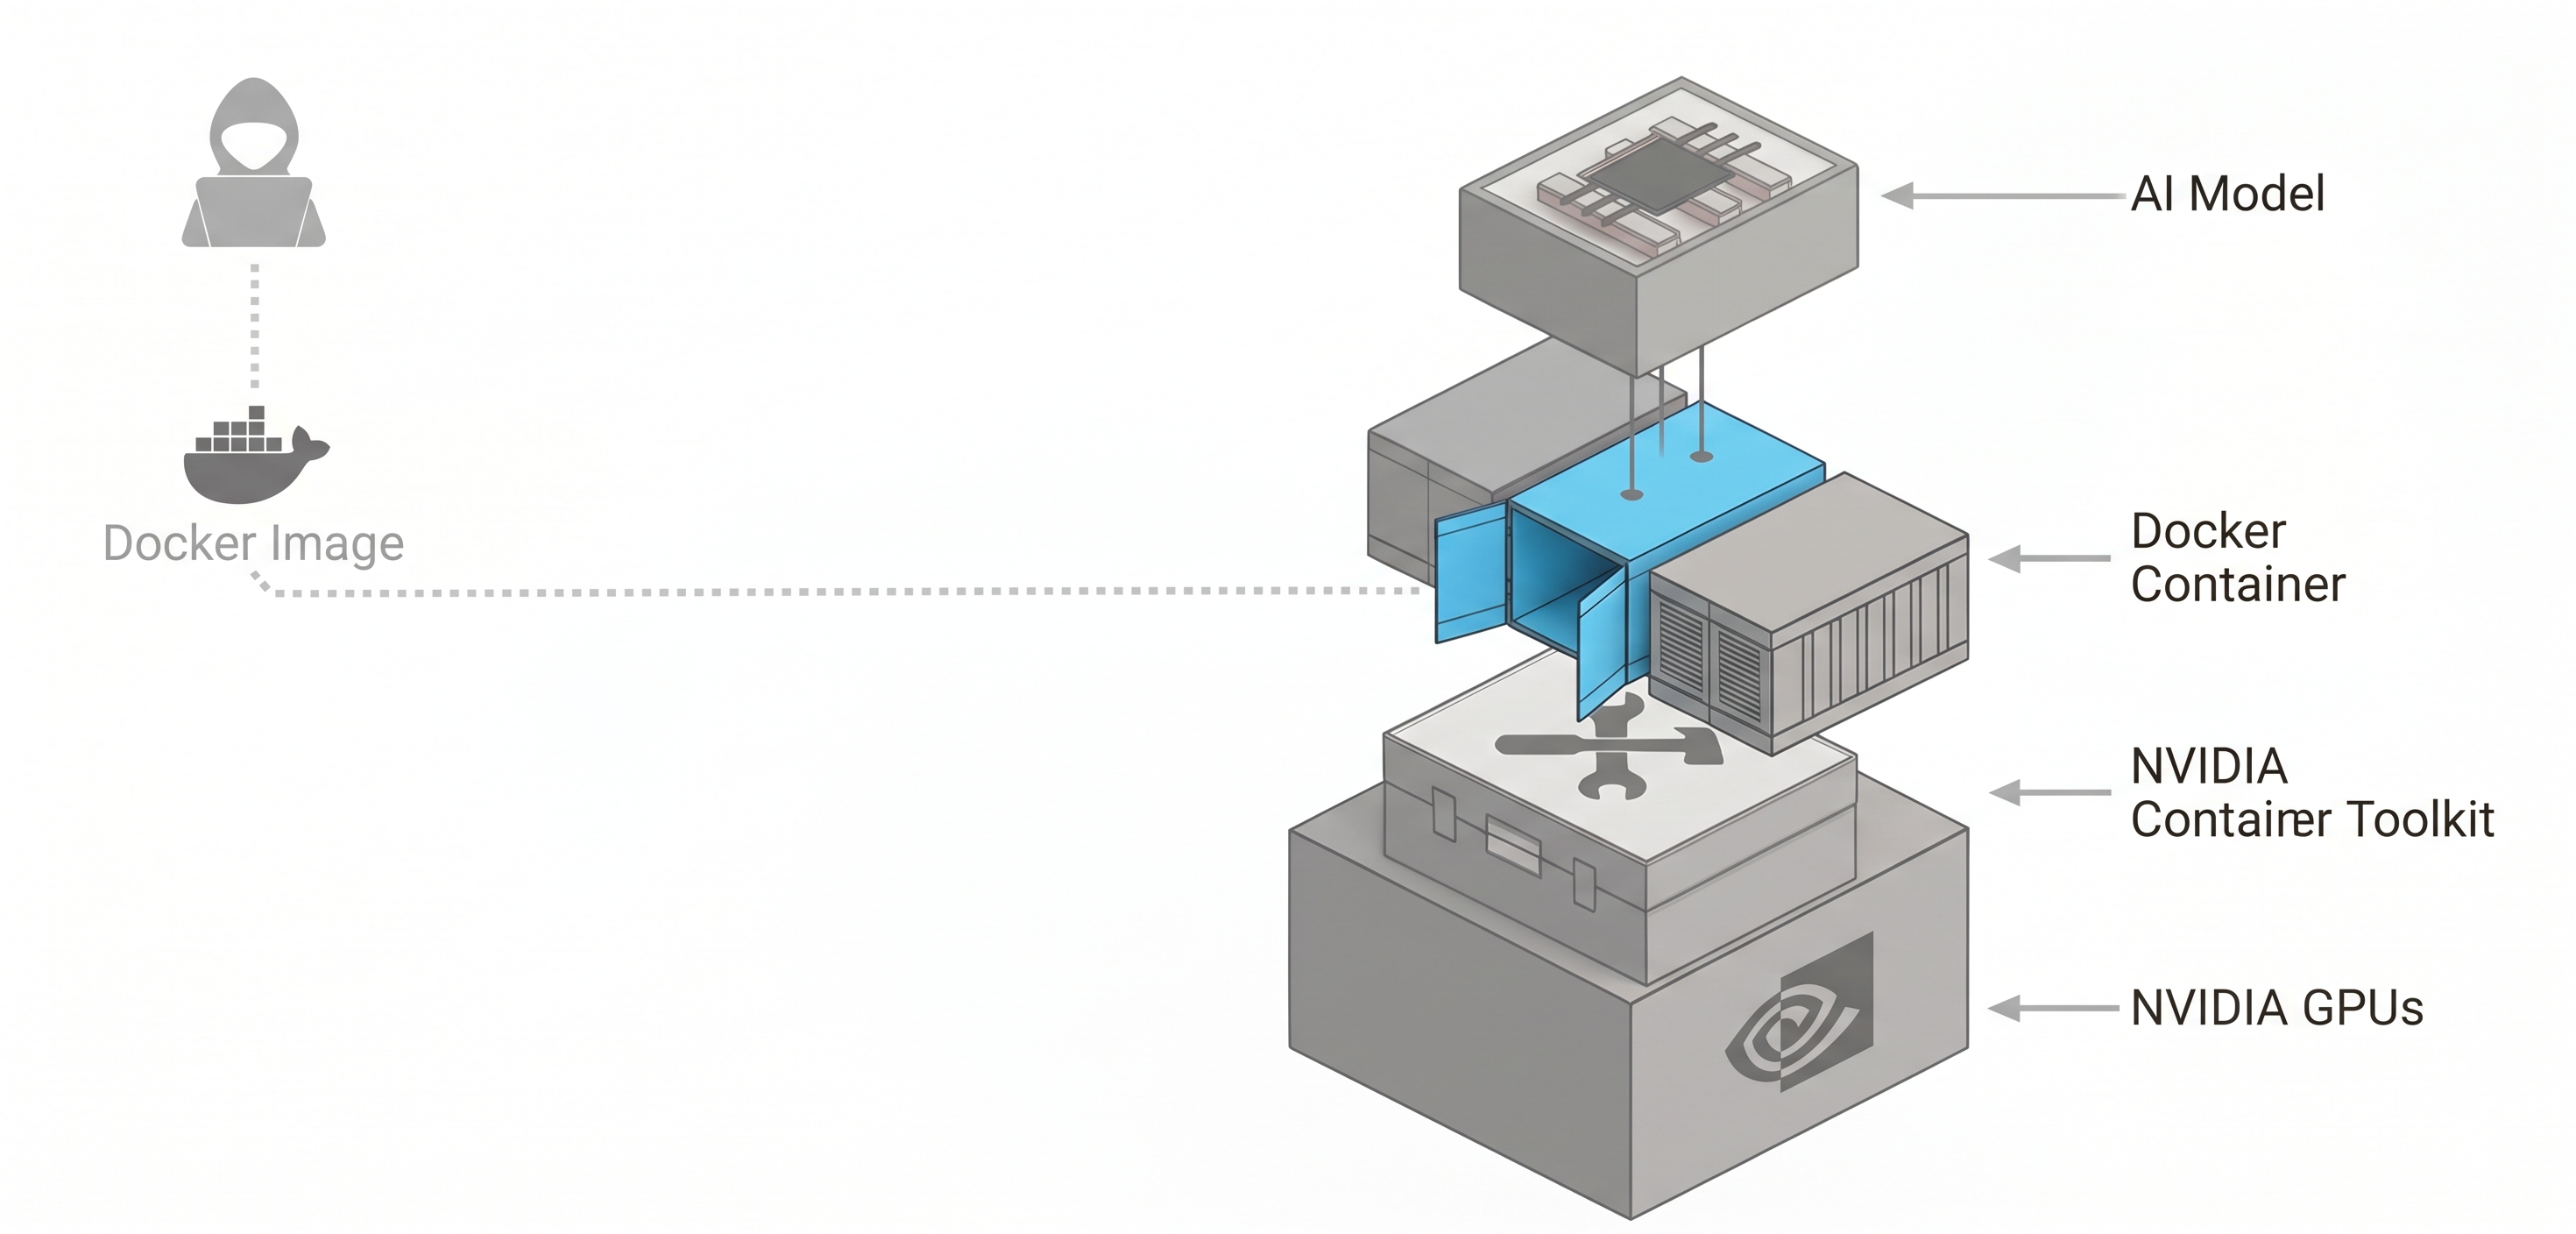
\includegraphics[width=\textwidth]{images/nvidiacontainer.png}
  \caption{NVIDIA Container Toolkit architecture and hook execution flow.}
  \label{fig:nvidia-container}
\end{figure}


\subsection{Root Cause: Unsafe Environment Inheritance}
\label{subsec:root-cause}

To understand the root cause precisely, we must examine how the OCI hook is invoked. When a container with GPU access is started, the container runtime (e.g., \texttt{runc} or \texttt{containerd}) reads the container's OCI bundle specification (\texttt{config.json}), which includes a list of hooks. The NVIDIA prestart hook entry looks approximately as follows:

\begin{lstlisting}[language=bash, caption={Simplified OCI hook specification for nvidia-ctk (config.json excerpt).}]
"hooks": {
  "prestart": [
    {
      "path": "/usr/bin/nvidia-ctk",
      "args": ["nvidia-ctk", "runtime", "hook", "prestart"],
      "env": []
    }
  ]
}
\end{lstlisting}

The OCI runtime specification states that hook processes receive the container's environment in the \texttt{env} field of the hook configuration. However, the problematic behaviour in the vulnerable versions of the toolkit arises from the fact that the hook process additionally inherits environment variables from its parent process (and the parent process's environment is populated, directly or indirectly, from the container's configured environment variables).
 
The crucial flaw is the absence of an explicit \texttt{execve()} call with a sanitised, minimal environment array before the hook begins its privileged operations \cite{linux_execve_manpage}. In Unix process semantics, \texttt{execve()} is the mechanism by which a process can replace its image with a new executable; critically, it accepts an explicit \texttt{envp} array, allowing the caller to specify a completely controlled environment for the new process. A correctly written privileged process that must execute in an environment derived from untrusted input would call \texttt{execve()} with a hand-crafted, minimal \texttt{envp} containing only the variables strictly necessary for operation.

The vulnerable toolkit does not perform this sanitisation. The \texttt{LD\_PRELOAD} variable, if present in the container's environment, propagates to the hook process where the dynamic linker acts upon it faithfully \cite{linux_ldso_manpage} (loading the attacker-specified library with root privileges).

\subsection{Attack Surface and Preconditions}
\label{subsec:attack-surface}

The attack surface of CVE-2025-23266 is defined by the following preconditions:

\begin{enumerate}
  \item \textbf{Vulnerable toolkit version}: The host must be running a version of the NVIDIA Container Toolkit prior to the patch. This affects a wide range of deployments that have not applied the security update.
  \item \textbf{GPU-enabled container}: The attacker must be able to start a container with GPU access (e.g., using the \texttt{-{}-gpus} flag in Docker or the \texttt{nvidia.com/gpu} resource request in Kubernetes). In shared cloud environments, this is a standard capability offered to paying customers.
  \item \textbf{Ability to set environment variables}: The attacker must be able to define environment variables for their container. This is universally true for any container a user controls.
  \item \textbf{Writable shared path}: The attacker's malicious shared library must be accessible to the host-side linker. This is achieved by placing the library in a path that is shared between the container and the host (such as a mounted volume or a device path accessible from both).
\end{enumerate}
 
Notably absent from this list are: kernel exploits, elevated container capabilities, network access, and any form of social engineering. The attack is self-contained within the container startup sequence.

\subsection{Exploit Walkthrough}
\label{subsec:exploit-walkthrough}

The following provides a conceptual, step-by-step walkthrough of the exploit chain.

\begin{enumerate}
  \item \textbf{Craft the malicious shared library.} The attacker writes a shared library containing a constructor function (a function annotated with \texttt{\_\_attribute\_\_((constructor))} in C) that executes the attacker's payload when the library is loaded. Because this runs before \texttt{main()}, it executes at the earliest possible moment in the host process lifecycle, before any security checks in the hook's application logic.
 
\begin{lstlisting}[language=C, caption={Pseudocode for the malicious shared library constructor.}]
// evil.c -- compiled to evil.so
#include <unistd.h>
#include <stdlib.h>
 
__attribute__((constructor))
void payload(void) {
    // Executed with root privileges on the HOST
    // at the moment the hook process loads this library.
    // Example: spawn a reverse shell, write an SSH key,
    // create a SUID shell binary, etc.
    system("/bin/bash -c 'cp /bin/bash /tmp/rootshell"
           " && chmod u+s /tmp/rootshell'");
}
\end{lstlisting}
 
  \item \textbf{Place the library on a shared path.} The library must be reachable from the host filesystem at the time the hook runs. The attacker mounts a host directory into their container (a common practice for data I/O) and writes the compiled \texttt{evil.so} there. Alternatively, certain NVIDIA device paths mounted by the toolkit itself may be exploitable.
 
  \item \textbf{Set \texttt{LD\_PRELOAD} in the container environment.} When starting the container, the attacker sets the environment variable \texttt{LD\_PRELOAD} to the host-side path of \texttt{evil.so}. In Docker CLI syntax:
 
\begin{lstlisting}[language=bash, caption={Container launch with injected LD\_PRELOAD.}]
docker run --gpus all \
  -e LD_PRELOAD=/mnt/shared/evil.so \
  -v /host/shared:/mnt/shared \
  attacker-image
\end{lstlisting}
 
  \item \textbf{Hook invocation.} As part of the container startup sequence, the OCI runtime invokes the NVIDIA prestart hook (\texttt{nvidia-ctk runtime hook prestart}) on the host with root privileges. Due to the environment inheritance vulnerability, \texttt{LD\_PRELOAD=/mnt/shared/evil.so} is present in the hook's environment.
 
  \item \textbf{Dynamic linker loads the malicious library.} The host's dynamic linker reads \texttt{LD\_PRELOAD} and maps \texttt{evil.so} into the hook process's address space before any standard libraries. The constructor function executes immediately.
 
  \item \textbf{Arbitrary code runs as root on the host.} The attacker's payload runs with the full privileges of the hook process (root on the host) achieving a complete container escape. The container itself need not even finish starting for the escape to succeed.
\end{enumerate}

The elegance of this exploit chain is its simplicity. No memory corruption, no kernel exploit, no race condition. A single environment variable and a compiled shared library are sufficient to escape the container and own the host.

\newpage
\section{Exploitation Mechanics}
\label{sec:exploitation}

\subsection{Injecting \texttt{LD\_PRELOAD} from the Container}
\label{subsec:injection}

The mechanics of environment variable injection deserve careful examination: In the OCI container model, environment variables are defined in two places: the container image's configuration (the \texttt{Env} field in the image manifest) \cite{oci_image_spec} and the runtime configuration provided at container launch (via \texttt{docker run -e} or Kubernetes \texttt{env} fields in a Pod specification \cite{k8s_security_docs}).
 
Both mechanisms ultimately result in the environment variables being written into the container's OCI \texttt{config.json} \cite{oci_runtime_spec}. The vulnerable NVIDIA toolkit versions propagate this environment to the hook process through the parent process chain without filtering \cite{nvidia_advisory_2025}. The following diagram illustrates the inheritance path:

\begin{lstlisting}[language=bash, caption={Environment propagation chain from container to privileged hook.}]
Container Runtime (dockerd / containerd)
    |
    |-- reads config.json (contains LD_PRELOAD set by attacker)
    |
    v
runc (OCI runtime) -> forks hook process
    |
    |-- inherits environment from runtime process
    |   (including LD_PRELOAD from container config)
    |
    v
nvidia-ctk hook [UID=0, running on HOST]
    |
    v
ld.so reads LD_PRELOAD -> loads evil.so -> constructor() executes
\end{lstlisting}

The key insight is that \texttt{runc} (or the equivalent runtime) spawns the hook process via \texttt{fork()} and \texttt{execve()}, but the \texttt{envp} argument passed to \texttt{execve()} (which should contain a clean, controlled environment) instead contains the attacker-influenced container environment.

\subsection{Privileged Hook Execution on the Host}
\label{subsec:hook-exec}

A critical aspect of the vulnerability is the privilege level at which the hook executes. OCI prestart hooks run in the host's mount namespace and with the full privilege set of the container runtime daemon, which is typically root \cite{oci_runtime_spec}. This is architecturally necessary: the hook must mount GPU device files into the container's namespace (an operation that requires \texttt{CAP\_SYS\_ADMIN} and the ability to interact with the host's device filesystem) \cite{linux_capabilities_manpage}.
 
What makes this particularly dangerous is that the hook runs \textit{before} the container's security policies (seccomp profiles, AppArmor policies, dropped capabilities) have been applied to the container process. The hook itself is not subject to the container's security configuration (it is a host process, not a container process \cite{nvidia_ctk_docs}).
 
Furthermore, in most production deployments, the NVIDIA Container Toolkit's hook binary is not subject to any additional Mandatory Access Control policy \cite{nvidia_advisory_2025}. It runs as a plain root process with full Linux capabilities, making it an extremely high-value target. Once the attacker's library is loaded into this process, there are effectively no further kernel-level restrictions preventing arbitrary host access.

\subsection{Escalation to Host Root}
\label{subsec:escalation}

The privilege escalation achieved through this vulnerability is immediate and unconditional. The constructor function in the malicious shared library executes in the security context of the \texttt{nvidia-ctk} hook process \cite{nvd_cve_2025_23266}, which means:
 
\begin{itemize}
  \item \textbf{UID 0 (root)} on the host system.
  \item \textbf{Full Linux capability set}, including \texttt{CAP\_SYS\_ADMIN}, \texttt{CAP\_DAC\_OVERRIDE}, \texttt{CAP\_CHOWN}, and all others \cite{linux_capabilities_manpage}.
  \item \textbf{Host mount namespace access}, allowing reading and writing of any file on the host filesystem \cite{linux_namespaces_manpage}.
  \item \textbf{Host network namespace access} (depending on how the runtime is configured), potentially enabling network-level attacks against other hosts.
\end{itemize}
 
Practical payloads an attacker could deploy include: writing an SSH public key to \texttt{/root/.ssh/authorized\_keys} for persistent access; creating a SUID copy of \texttt{/bin/bash} in a world-writable directory, modifying \texttt{/etc/passwd} or \texttt{/etc/sudoers} to add an unprivileged account with root access, installing a kernel rootkit or exfiltrating sensitive host secrets (API keys, TLS certificates, other container data) \cite{wiz_nvidia_2024}.

\subsection{Realistic Attack Scenario: Cloud Multi-Tenant AI}
\label{subsec:scenario}

To contextualise the real-world severity of NVIDIAScape, consider the following realistic attack scenario in a cloud AI infrastructure:
 
\paragraph{Setting.} A cloud provider offers GPU-accelerated compute instances for AI model training and inference. Multiple customers share the same physical host, each running their workloads in isolated containers. The host runs the NVIDIA Container Toolkit (vulnerable version) to provide GPU access to all tenants.
 
\paragraph{Attacker.} A malicious customer (Tenant A) provisions a standard GPU container instance (a service available to any paying customer with no special vetting). They have full control over their container's environment variables and can mount volumes.
 
\paragraph{Attack sequence.}
\begin{enumerate}
  \item Tenant A writes a malicious shared library (\texttt{evil.so}) implementing a reverse shell or a persistent backdoor into a volume accessible from the host.
  \item Tenant A starts their container with \texttt{LD\_PRELOAD} pointing to \texttt{evil.so}.
  \item The NVIDIA hook executes on the host, loads \texttt{evil.so}, and the payload runs as root.
  \item The attacker now has root on the host. They can: read the memory, disk, and GPU state of all other tenants on the same host, exfiltrate proprietary model weights from Tenant B's running container, extract API keys and credentials from environment variables of other containers, pivot to the cloud provider's internal network via the host's network interfaces.
\end{enumerate}
 
\paragraph{Impact.} The breach extends far beyond the attacker's own container. All co-located tenants are compromised, the cloud provider's infrastructure is at risk, and the attacker has achieved lateral movement potential into the provider's broader internal network. \cite{nvd_cve_2025_23266, wiz_nvidia_2024}.
 Remember that all these problems started from a standard, unprivileged GPU container.

\newpage
\section{Impact Assessment}
\label{sec:impact}

% ~3.000 characters total across subsections

\subsection{CVSS Score and Breakdown}
\label{subsec:cvss}

CVE-2025-23266 carries a \textbf{CVSS v3.1 Base Score of 9.0 (Critical)} \cite{nvd_cve_2025_23266, cvss_v31_spec}. The breakdown of the vector string is as follows:
 
\begin{table}[H]
\centering
\caption{CVSS v3.1 Vector Breakdown for CVE-2025-23266}
\label{tab:cvss}
\begin{tabularx}{\textwidth}{lXl}
\toprule
\textbf{Metric} & \textbf{Description} & \textbf{Value} \\
\midrule
Attack Vector (AV) & Attacker must have local access (inside a container) & Local (L) \\
Attack Complexity (AC) & No special conditions; attack is reliably repeatable & Low (L) \\
Privileges Required (PR) & Standard container user, no elevated privileges needed & Low (L) \\
User Interaction (UI) & No victim interaction required; purely automated & None (N) \\
Scope (S) & Impact escapes the vulnerable component (container) & Changed (C) \\
Confidentiality (C) & Complete host confidentiality loss & High (H) \\
Integrity (I) & Complete host integrity loss & High (H) \\
Availability (A) & Host availability can be fully disrupted & High (H) \\
\bottomrule
\end{tabularx}
\end{table}

The \textbf{(Metric = Scope, Value = Changed)} tuple is particularly noteworthy. It reflects the fact that the vulnerability's impact transcends the security boundary of the initially vulnerable component (the container) and affects a separate, higher-privilege component (the host). This scope change is the defining characteristic of a container escape vulnerability and is the primary driver of the high base score.

\subsection{Impact on Kubernetes and Docker GPU Environments}
\label{subsec:k8s-impact}

The vulnerability has significant implications across the two dominant GPU container deployment platforms.

\paragraph{Docker.} In a standard Docker deployment with GPU support, the attack is straightforward as described in the exploit walkthrough (\ref{subsec:exploit-walkthrough}). Any user with the ability to run GPU-enabled containers on a host with the vulnerable toolkit can exploit the vulnerability. In practice, Docker is widely used for development workstations, on-premises GPU servers, and small-scale cloud deployments \cite{nvd_cve_2025_23266}.
 
\paragraph{Kubernetes.} The impact in Kubernetes environments is potentially broader and more severe \cite{k8s_security_docs}. In a Kubernetes cluster with GPU node pools, the NVIDIA Container Toolkit is deployed as a DaemonSet on GPU nodes, making it universally present on all GPU-capable nodes \cite{k8s_device_plugin}. An attacker who can submit a Pod specification with GPU resource requests and arbitrary environment variables (which is a standard capability for any authenticated Kubernetes user with access to a GPU namespace) can exploit the vulnerability on any GPU node the pod is scheduled on.

Moreover, Kubernetes introduces additional blast-radius concerns:
\begin{itemize}
  \item The compromised node's \texttt{kubelet} credentials can be extracted, potentially enabling lateral movement to the Kubernetes API server.
  \item The node's service account tokens mounted into pods can be used to interact with the cluster's API.
  \item In cloud-managed Kubernetes services (GKE, EKS, AKS), the node's cloud instance metadata endpoint may be accessible, potentially yielding cloud IAM credentials with broad permissions.
\end{itemize}

\subsection{Risk for LLM and AI Hosting Infrastructure}
\label{subsec:ai-risk}

The intersection of NVIDIAScape with modern AI infrastructure deserves particular emphasis. The past several years have seen explosive growth in GPU-enabled container deployments driven by large language model (LLM) training and inference workloads. Organisations such as cloud providers, AI startups, and research institutions routinely operate dense GPU clusters where many tenants share physical nodes.
 
In this context, the threat model for NVIDIAScape is especially concerning for the following reasons:
 
\paragraph{High-value targets on GPU nodes.} GPU nodes hosting LLM inference typically contain: proprietary model weights (often representing millions of dollars in training costs), API keys and secrets injected via environment variables into inference containers, customer data submitted for inference, and billing and identity information. A container escape on such a node yields immediate access to all of this.
 
\paragraph{Shared GPU nodes in inference clusters.} Large-scale LLM serving infrastructure frequently uses bin-packing strategies that place multiple customer workloads on the same GPU node to maximise utilisation. This maximises the value of a single successful container escape.
 
\paragraph{Automated and autoscaling deployments.} The automated nature of cloud-native GPU deployments means that vulnerable nodes may be continuously provisioned and deprovisioned without manual security review. Unless patch deployment is automated, vulnerable versions can persist in production for extended periods.
 
\paragraph{Regulatory and compliance implications.} Organisations in regulated industries (healthcare, finance) that use GPU cloud infrastructure for AI workloads face additional exposure from NVIDIAScape: a successful exploit could result in cross-tenant data leakage that triggers data breach notification obligations under GDPR, HIPAA, or SOC 2 requirements.

\newpage
\section{Mitigation and Hardening}
\label{sec:mitigation}

\subsection{NVIDIA's Official Patch}
\label{subsec:patch}

NVIDIA released a patched version of the Container Toolkit that directly addresses the environment variable inheritance flaw. The fix introduces explicit environment sanitisation in the hook process startup path. Specifically, the patched code constructs a minimal, explicitly defined environment array before executing the hook's privileged operations, ensuring that variables such as \texttt{LD\_PRELOAD}, \texttt{LD\_LIBRARY\_PATH}, \texttt{LD\_AUDIT}, and other dynamic linker control variables are stripped from the hook's execution environment regardless of what the container configuration specifies.
 
\paragraph{Recommended action.} All operators of GPU-enabled container infrastructure should immediately upgrade the NVIDIA Container Toolkit to the patched version.\\ The upgrade process involves the \texttt{libnvidia-container}, \texttt{nvidia-container-toolkit}, and \texttt{nvidia-container-runtime} packages and restarting the container runtime daemon.

\begin{lstlisting}[language=bash, caption={Package upgrade commands for common Linux distributions.}]
# Debian/Ubuntu
sudo apt-get update
sudo apt-get install -y nvidia-container-toolkit
sudo systemctl restart docker  # or containerd
 
# RHEL/CentOS/Rocky Linux
sudo dnf update nvidia-container-toolkit
sudo systemctl restart docker
 
# Verify installed version
nvidia-ctk --version
\end{lstlisting}
 
\paragraph{In Kubernetes.} The toolkit DaemonSet must be updated on all GPU nodes. Depending on the cluster configuration, this may require a node drain cycle to safely restart the container runtime without disrupting running GPU workloads.

\paragraph{CDI mode as architectural mitigation.}
As a complementary measure, operators should evaluate migrating to the Container Device Interface (CDI) mode supported by recent versions of the NVIDIA Container Toolkit. CDI decouples device configuration from the OCI hook execution path: instead of a privileged hook running at container startup, device specifications are pre-generated on the host and consumed by the runtime as static configuration \cite{cdi_spec}. This removes the dynamic hook invocation entirely, eliminating the environment inheritance vector at an architectural level.

\subsection{Applying the Principle of Least Privilege}
\label{subsec:least-privilege}

Beyond patching the immediate vulnerability, the NVIDIAScape case highlights the importance of applying the \textbf{Principle of Least Privilege} (\textbf{PoLP}) to privileged system toolkit components \cite{nist_sp800_190}.
 
The \texttt{nvidia-ctk} hook needs root access to perform specific, well-defined operations: mounting device files, configuring cgroups, and setting up library bind mounts. Rather than running as unrestricted root, a hardened implementation would:
 
\begin{itemize}
  \item Use a minimal capability set, retaining only those capabilities strictly required (e.g., \texttt{CAP\_SYS\_ADMIN} for mount operations, \texttt{CAP\_DAC\_OVERRIDE} for device file access) and dropping all others explicitly via \texttt{cap\_set\_proc()}.
  \item Execute as a dedicated, non-login service account rather than the system root user, even when elevated capabilities are required.
  \item Implement privilege separation, performing privileged operations in a short-lived child process that immediately exits after completing its specific task, rather than maintaining elevated privileges throughout the hook's lifecycle.
\end{itemize}

\subsection{Environment Sanitisation at execve()}
\label{subsec:env-sanitisation}

The technically correct fix at the code level (independent of the NVIDIA-specific patch) is the application of environment sanitisation at the \texttt{execve()} boundary. Any program that must execute with privileges derived from a context that includes untrusted environment variables should adopt the following pattern:
 
\begin{lstlisting}[language=C, caption={Correct environment sanitisation pattern using execve() with explicit envp.}]
#include <unistd.h>
 
// Safe environment: only variables the hook legitimately needs
char *safe_env[] = {
    "PATH=/usr/local/sbin:/usr/local/bin:/usr/sbin:/usr/bin:/sbin:/bin",
    NULL  // Terminator
};
 
// Re-execute self (or the actual hook binary) with clean environment
execve("/proc/self/exe", argv, safe_env);
// If execve returns, it failed -> handle the error
perror("execve");
exit(EXIT_FAILURE);
\end{lstlisting}
 
This pattern is analogous to what Set-UID programs effectively benefit from automatically via the dynamic linker's \texttt{AT\_SECURE} flag. By explicitly constructing the environment, the hook author removes any dependency on inherited state from untrusted sources.
 
An alternative approach is to use \texttt{clearenv()} to remove all environment variables and then re-add only those explicitly required. However, the \texttt{execve()} re-execution pattern is generally considered more robust, as it also eliminates any state that may have been inherited in process-internal structures (file descriptors, signal masks, etc.).

\subsection{Defence-in-Depth}
\label{subsec:defense-in-depth}

Patching the toolkit and sanitising execution environments address the specific vulnerability, but a robust security posture requires defence-in-depth \cite{nist_sp800_190} (multiple independent layers of controls that limit the impact of any single failure).
 
\paragraph{Seccomp profiles.} The \texttt{nvidia-ctk} hook process should be subject to a restrictive seccomp profile that allows only the system calls strictly necessary for its GPU configuration operations. At a minimum, this profile should block \texttt{execve()} with arbitrary arguments, preventing the hook from spawning attacker-controlled child processes. Docker and Kubernetes support custom seccomp profiles that can be applied to specific components \cite{docker_seccomp} \cite{k8s_security_docs}.
 
\paragraph{AppArmor / SELinux policies.} Mandatory Access Control frameworks can confine the hook process to a specific, minimal set of filesystem paths and operations. An AppArmor profile for \texttt{nvidia-ctk} would, for example, allow writes only to specific \texttt{/dev/nvidia*} paths and the container's rootfs device mount points, while denying writes to sensitive host paths such as \texttt{/root}, \texttt{/etc}, and \texttt{/home} \cite{apparmor_ubuntu}.
 
\paragraph{Rootless containers.} Running the container runtime in rootless mode (where the container runtime itself operates as an unprivileged user) significantly reduces the blast radius of hook-based attacks. In rootless mode, the hook process does not have true root privileges on the host, and its ability to affect host-wide state is constrained. While GPU support for rootless containers has historically been limited, recent versions of the NVIDIA toolkit have improved rootless GPU support.
 
\paragraph{Read-only and no-new-privileges flags.} Containers should be started with the \texttt{no-new-privileges} security option whenever possible. While this does not directly prevent NVIDIAScape (the exploit occurs in the hook, not the container process), it limits the post-escape options available to an attacker if they attempt to escalate further from within the container.
 
\paragraph{Network segmentation and egress filtering.} Even if an attacker achieves host root, network-level controls can limit the damage. Strict egress filtering on GPU nodes (allowing only expected outbound connections) can prevent reverse shells and data exfiltration attempts from succeeding, buying time for incident response.

\newpage
\section{Broader Implications}
\label{sec:implications}

\subsection{Set-UID Architecture vs Service-Based Design}
\label{subsec:setuid-vs-service}

The NVIDIAScape vulnerability illuminates a fundamental architectural tension in the design of privileged system software. Two broad paradigms exist for components that must perform privileged operations on behalf of unprivileged callers:
 
\paragraph{Set-UID / Direct Execution Model.} In this model, a binary is given elevated privileges via the Set-UID bit or capabilities, and is invoked directly by the unprivileged caller. The binary runs in an environment largely inherited from the caller. Security depends entirely on the binary's own defences (proper environment sanitisation, capability dropping, input validation, and so forth). The dynamic linker provides one automatic protection (\texttt{AT\_SECURE}) for SUID binaries, but this does not cover all inheritance paths. Historical experience shows that SUID programs are a persistent source of privilege escalation vulnerabilities.
 
\paragraph{Service / IPC Model.} In this model, the privileged operations are performed by a long-running daemon (a service) that runs as root or with specific capabilities, and that receives requests from unprivileged clients via a well-defined inter-process communication (IPC) channel (Unix socket, D-Bus, etc.). This model is architecturally more secure because the trust boundary is explicit: the service validates each incoming request independently of the caller's environment.
 
The \texttt{nvidia-ctk} hook architecture is closer to the Set-UID model: it is invoked directly, inheriting environmental state from the runtime chain. Had the GPU toolkit been designed as a privileged service (e.g., a Unix socket daemon receiving structured hook invocation requests), the \texttt{LD\_PRELOAD} injection vector would not exist.
 
This architectural lesson is broadly applicable: system-level toolkits that bridge unprivileged workloads and privileged hardware or OS resources should prefer service-based designs over direct invocation models wherever feasible.

\subsection{System Toolkits as Attack Vectors}
\label{subsec:toolkits-as-vectors}

CVE-2025-23266 is a reminder that \textbf{the software infrastructure around containers is as much a part of the attack surface as the containers themselves}. The security community's focus on container hardening is valuable but incomplete if the privileged components of the container ecosystem are not equally rigorous.
 
Hardware management layers (GPU drivers, storage drivers, network plugins, device plugins in Kubernetes) represent a particularly attractive attack surface for several reasons:
 
\begin{itemize}
  \item They are maintained by hardware vendors whose primary expertise is hardware enablement, not security engineering.
  \item They require deep integration with the operating system, often necessitating elevated privileges that the container runtime itself does not require.
  \item They are frequently treated as trusted infrastructure, exempt from the security scrutiny applied to application containers.
  \item Their update cadence may lag behind security disclosures, particularly in regulated or conservative enterprises.
\end{itemize}
 
The practical implication is that security teams responsible for container infrastructure must extend their threat models to include the privileged toolkit layer. Vulnerability scanning tools should explicitly track versions of container toolkits and plugins alongside the container runtime and kernel versions. Security-sensitive deployments should have explicit policies for toolkit update response times following CVE disclosure.

\subsection{The Future of GPU Security in AI Infrastructure}
\label{subsec:gpu-security-future}

The trajectory of AI infrastructure development suggests that the attack surface represented by NVIDIAScape will grow rather than shrink in the coming years.
 
\paragraph{Increasing GPU density and multi-tenancy.} As GPU compute becomes more expensive and in demand, infrastructure providers will continue to maximise hardware utilisation through dense multi-tenancy. This amplifies the impact of any single container escape, making individual vulnerabilities more consequential.
 
\paragraph{MIG and GPU partitioning.} NVIDIA's Multi-Instance GPU (MIG) technology allows a single physical GPU to be partitioned into multiple isolated instances for simultaneous use by different workloads. While MIG provides hardware-level isolation between GPU workloads, the Container Toolkit still manages the host-side configuration of MIG instances (meaning that vulnerabilities in the toolkit remain relevant even in MIG deployments \cite{nvidia_mig_docs}).
 
\paragraph{Confidential computing for AI.} The emerging field of confidential computing aims to provide cryptographic isolation of workloads even from the host operator. NVIDIA's Confidential Computing mode encrypts GPU memory and attestation state, making it inaccessible to the host. However, the Container Toolkit must still interface with the host to configure confidential GPU instances, and vulnerabilities in this configuration path remain a potential concern \cite{nvidia_confidential_compute}.
 
\paragraph{Supply chain security.} As AI infrastructure becomes critical infrastructure, the security of the supply chain for GPU management software will attract increasing attention from both defenders and attackers. Code signing, reproducible builds, and formal security reviews for toolkit releases will become more important \cite{nvidia_ctk_github}.
 
\paragraph{Regulatory pressure.} Emerging AI regulation increasingly mandates security controls for AI systems that process sensitive data. This will drive demand for formal security assessments of GPU infrastructure components, including container toolkits, and may accelerate the adoption of secure-by-design architectural patterns\cite{eu_ai_act}.
 
In summary, NVIDIAScape is not an anomaly but a leading indicator of a broader challenge: securing the privileged software infrastructure that connects AI workloads to the physical hardware they depend on. Meeting this challenge requires architectural improvements in toolkit design, rigorous vulnerability management programs, and a security posture that treats the container toolchain as a first-class threat surface.

\newpage
\section{Conclusion}
\label{sec:conclusion}

This paper has presented a comprehensive analysis of NVIDIAScape (CVE-2025-23266), a critical container escape vulnerability arising from unsafe environment variable inheritance in the NVIDIA Container Toolkit's privileged OCI hook. We have examined the technical root cause (the absence of environment sanitisation at the \texttt{execve()} boundary) and traced the precise exploit chain by which an attacker within an unprivileged container can achieve arbitrary code execution with root privileges on the host.
 
The vulnerability exemplifies a class of security failures that recurs across the history of privileged system software: the unsafe consumption of untrusted input inherited through the process execution chain. In this specific case, the inherited input is the \texttt{LD\_PRELOAD} environment variable, and the dynamic linker's faithful processing of it becomes the mechanism of exploitation. The exploit requires no kernel vulnerability, no elevated container permissions, and no user interaction, only a standard GPU container and control over its environment variables.
 
The impact in modern AI infrastructure is severe. GPU nodes hosting multi-tenant LLM workloads represent some of the most data-rich and commercially sensitive targets in current cloud infrastructure, and the ubiquity of the NVIDIA Container Toolkit across GPU deployments means that the vulnerability had a very broad blast radius at the time of disclosure.
 
Several lessons emerge from this analysis. First, privileged system toolkits must treat their execution environment as untrusted when that environment is derived, directly or indirectly, from unprivileged input. Second, the Principle of Least Privilege must be applied not only to container workloads but equally to the privileged components of the container ecosystem itself. Third, service-based architectural designs for hardware management layers are inherently more robust than direct invocation models that inherit caller state. Fourth, defence-in-depth controls (Mandatory Access Control policies, seccomp profiles, rootless container runtimes) provide critical residual protection when individual components fail.
 
As AI workloads continue to demand GPU resources at scale, and as the infrastructure supporting them grows in complexity and strategic value, the security of the privileged software layer connecting containers to hardware will remain a critical and underexplored frontier. NVIDIAScape is a precise and instructive case study in both the fragility of this layer and the clear engineering principles that can make it more robust.

% ─── References ──────────────────────────────────────────────────────────────
\nocite{*}
\printbibliography[heading=bibintoc, title={References}]

\end{document}